\subsubsection{Rationale/Context}

Any traveller might want to cancel their reserved trip to one of the islands. Of course, they can do that until one week before the departure date. If the reservation is cancelled they would receive their money back minus the administration fees.

\subsubsection{User story}

As an employee, I want to cancel a certain reservation.

\subsubsection{Use Case}
\creator{\studentC}
\updater{\studentA}
\secondUpdater{\studentB}

\textbf{Use Case Name:} Delete a trip reservation

\textbf{Scope:} Reservations system

\textbf{Level:} User Goal

\textbf{Primary Actor:} KOENDES Employee

\textbf{Stakeholders and Interests:} 
\begin{itemize}
\item \textit{Stakeholder:} KOENDES Employee (Wants an easy and quick process)
\item \textit{Stakeholder:} Traveller (Wants to cancel the reservation)
\end{itemize}

\textbf{Preconditions:} 
\begin{itemize}
\item The reservation exists in the system.
\item The departure date is more than a week after the cancellation request's date.
\item The user is an employee and authorised to make cancellations.
\end{itemize}

\textbf{Success Guarantee (Postconditions):}
\begin{itemize}
\item State change: The reservation has been deleted if the departure date is more than a week after; otherwise it is not deleted and the user gets informed.
\item Output: "Sorry the reservation cannot be cancelled." if the departure date is within one week; otherwise "The reservation has been cancelled!".
\end{itemize}

\textbf{Main Success Scenario (Basic Flow):}
\begin{enumerate}
\item The user asks the system to find a reservation
\item The system sends the user an empty search form for reservations
\item The user enters the reservation's number provided by traveller.
\item The user sends the filled form to the system.
\item The system sends back the reservation that matches the search query.
\item The user asks the system to delete the reservation.
\item The system deletes the reservation if that was possible.
\item The system calculates the refund amount to be the total amount paid minus administration fees.
\item The system sends the refund to the traveller.
\item The system informs the user with the final result.
\end{enumerate}
Extensions:
\begin{enumerate}
\item[7a] The reservation cannot be cancelled if the request is within one week before departure. So the system informs the user that it could not be deleted.
\end{enumerate}
\textbf{Technology And Data Variations List:} 
\begin{itemize}
    \item Last name: String with alphabetical characters only
    \item Reservation date: Date of the form DD/MM/YYYY
    \item Reservation's number: Numerical string
\end{itemize}
\textbf{Frequency of Occurrence:}
\begin{itemize}
    \item Only a few times per month.
\end{itemize}
\subsubsection{SSD}
\creator{\studentC}
\updater{\studentA}
\secondUpdater{\studentB}\\
Considering the previous sub-sections we can create the following SSD model:\\\\
User $\rightarrow$ System: FindReservation;\hfill /* 1\\
System $\rightarrow$ User: Empty reservations search form;\hfill /* 2\\
User $\rightarrow$ User: Inserting (Reservation Number) to the form;\hfill /* 3\\
User $\rightarrow$ System: Filled-in search form;\hfill /* 4\\
System $\rightarrow$ User: The reservation that matches the search query with its (Reservation ID);\hfill /* 5\\
User $\rightarrow$ System: DeleteReservation(Reservation ID);\hfill /* 6\\
if Reservation has a departure date more than 1 week after\\
then System $\rightarrow$ System: Delete Reservation;\hfill /* 7\\
\phantom{x}\hspace{2ex}System $\rightarrow$ System: RefAmount(Reservation ID) = TotalAmount - AdministrationFees;\hfill /* 8\\
\phantom{x}\hspace{2ex}System $\rightarrow$ System: RefundToTraveller(RefAmount);\hfill /* 8\\
\phantom{x}\hspace{2ex}System $\rightarrow$ User: "The reservation has been cancelled!"\hfill /* 9\\
\phantom{x}\hspace{2ex}fi;\\
else System $\rightarrow$ User: "Sorry the reservation cannot be cancelled."\hfill /* 7a\\
fi;\\
%\includegraphics[scale=0.9]{UC1}
\newpage
\subsubsection{Grey box SD}
\creator{\studentB}
\updater{\studentC}
\begin{figure}[H]
    \centering
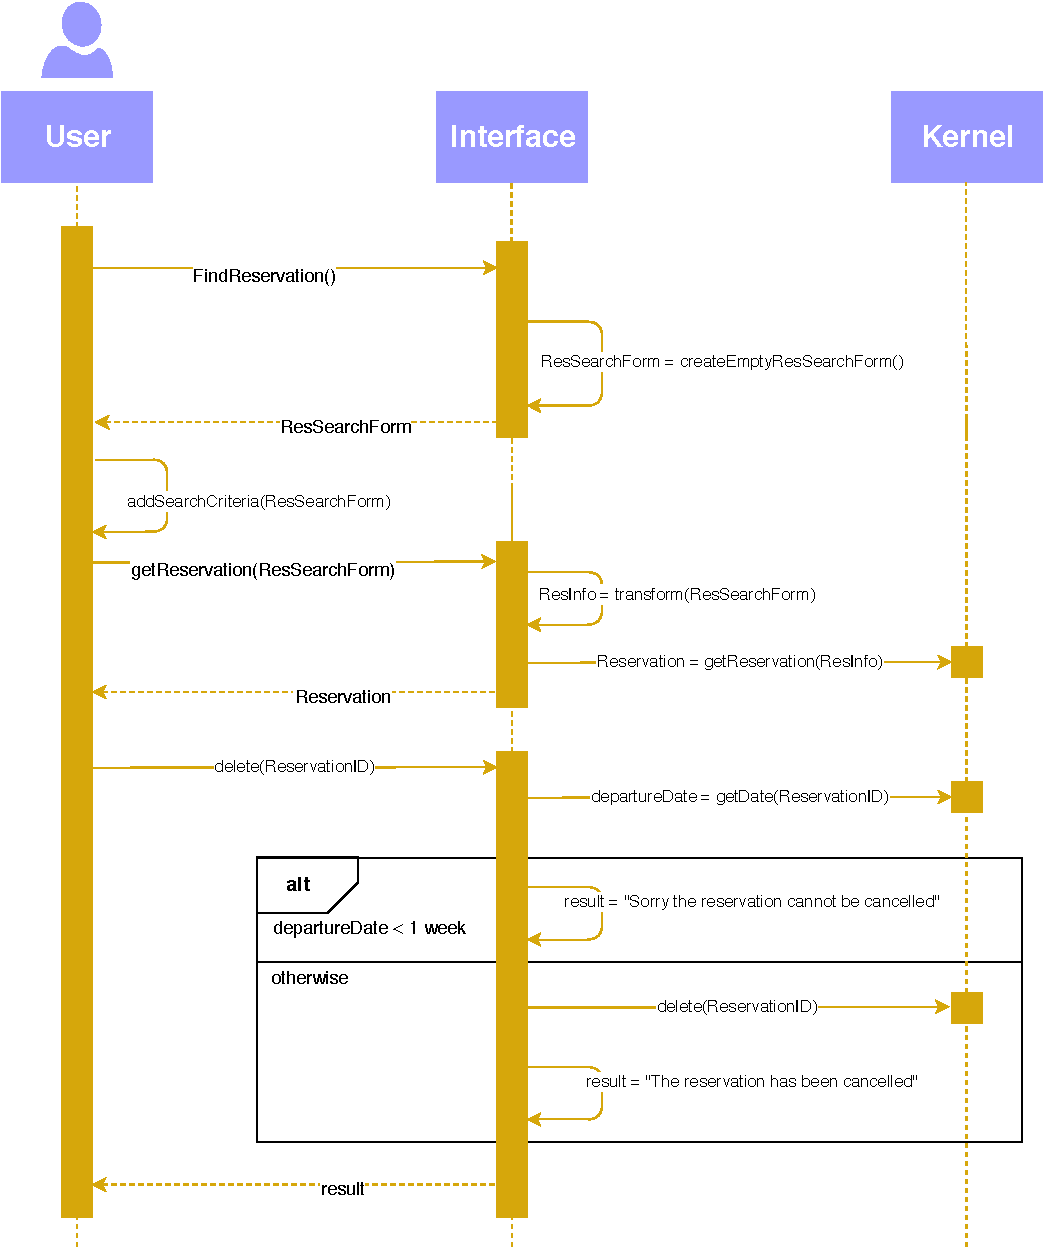
\includegraphics[scale=0.7]{Iteration_3/Files/UC3_gb.pdf}
    \caption{6.3 Grey box}
    \label{fig:6.3 Greybox}
\end{figure}

\subsubsection{White box SD}
\creator{\studentB}
\updater{\studentC}
\begin{figure}[H]
    \centering
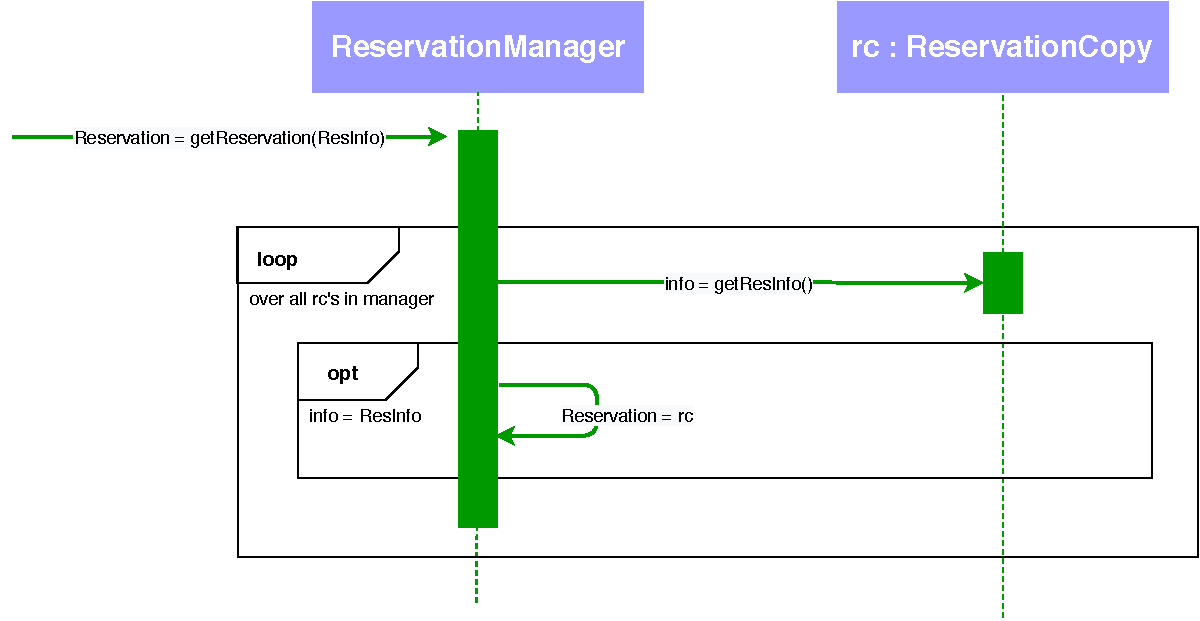
\includegraphics[scale=0.65]{Iteration_3/Files/UC3_wb1.pdf}
\end{figure}
\begin{figure}[H]
    \centering
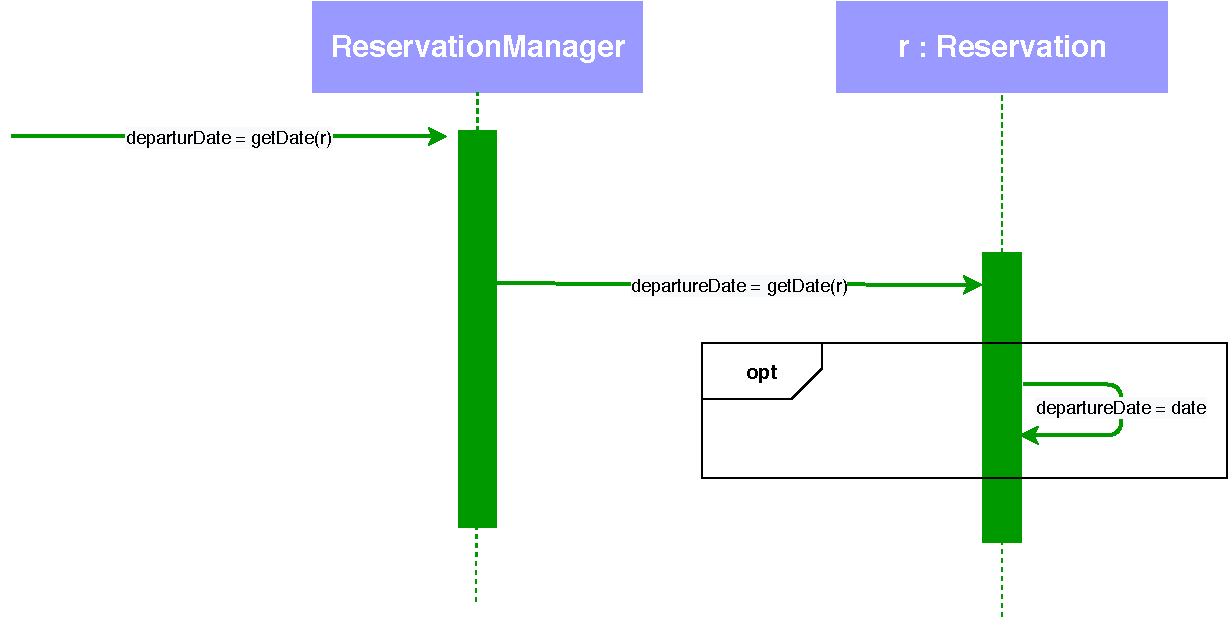
\includegraphics[scale=0.65]{Iteration_3/Files/UC3_wb3.pdf}
\end{figure}
\begin{figure}[H]
    \centering
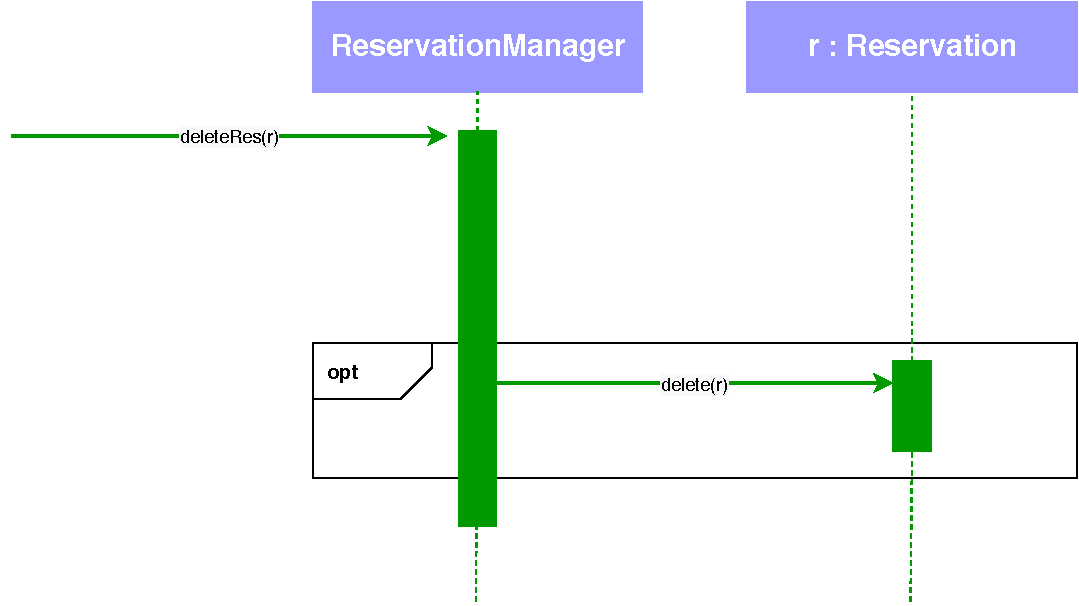
\includegraphics[scale=0.65]{Iteration_3/Files/UC3_wb2.pdf}
\end{figure}

%\includegraphics[scale=0.9]{UC1wb.pdf}

%\subsubsection{Design Considerations}